\documentclass[a4paper,14pt]{article} % формат документа

\usepackage{cmap} % поиск в ПДФ
\usepackage[T2A]{fontenc} % кодировка
\usepackage[utf8]{inputenc} % кодировка исходного текста
\usepackage[english,russian]{babel} % локализация и переносы
\usepackage[left = 2cm, right = 1cm, top = 2cm, bottom = 2 cm]{geometry} % поля
\usepackage{listings}
\usepackage{graphicx} % для вставки рисунков
\usepackage{amsmath}
\graphicspath{{pictures/}}
\DeclareGraphicsExtensions{.pdf,.png,.jpg}
\newcommand{\anonsection}[1]{\section*{#1}\addcontentsline{toc}{section}{#1}}

\lstset{ %
	language=Python,                % Язык программирования 
	numbers=left,                   % С какой стороны нумеровать          
	frame=single,                    % Добавить рамку
}

\begin{document}
	\begin{titlepage}

       		\begin{center}
         		\large
		
        			Государственное образовательное учреждение высшего профессионального образования\\
       			“Московский государственный технический университет имени Н.Э.Баумана”
         		\vspace{3cm}
            
            		\textsc{Дисциплина: Анализ алгоритмов}
           		\vspace{0.5cm}
                
            		\textsc{Лабораторная работа № 3}
           		 \vspace{3cm}
            
           		 \LARGE 
		 
		 	Трудоемкость алгоритмов сортировок
           		 \vspace{3cm}
            
            		\begin{flushright}
            			Студент: \\
				Сиденко Анастасия Генадьевна \\   
            			Группа: ИУ7-53Б \\
           			\hfill
            
           			Преподаватели: \\
				Строганов Юрий Владимирович \\
           			Волкова Лилия Леонидовна
            			\vfill
            		\end{flushright}
		
			\large
            		2019 г.
		\end{center}

	\end{titlepage}
    
	\tableofcontents
	
	\newpage
    
	\anonsection{Введение}
	\hfill
	
	Алгоритмы сортировки имеют большое практическое применение. Их можно встретить почти везде, где речь идет об обработке и хранении больших объемов информации. Сортировки используются в самом широком спектре задач, включая обработку коммерческих, сейсмических, космических и прочих данных[1]. Часто сортировка является просто вспомогательной операцией для упорядочивания данных, упрощения последующих алгебраических действий над данными и т.п.
	
	\hfill
	
	Сортировка применяется во всех без исключения областях программирования, например, базы данных или математические программы. Упорядоченные объекты содержатся в телефонных книгах, ведомостях налогов, в библиотеках, в оглавлениях, в словарях. 
	
	\hfill
	
	В учебнике [2, стр. 21] Д. Кнута упоминается что «по оценкам производителей компьютеров в 60-х годах в среднем более четверти машинного времени тратилось на сортировку. Во многих вычислительных системах на нее уходит больше половины машинного времени. Исходя из этих статистических данных, можно заключить, что либо (i) сортировка имеет много важных применений, либо (ii) ею часто пользуются без нужды, либо (iii) применяются в основном неэффективные алгоритмы сортировки». 
	
	\hfill
	
	В настоящее время, в связи с экспоненциально возросшими объемами данных, вопрос эффективной сортировки данных снова стал актуальным.
	
	\hfill
	
	К примеру, на сайте [3] можно найти результаты производительности алгоритмов сортировки для ряда ведущих центров данных. При этом используются различные критерии оценки эффективности. 
	
	\hfill
	
	В данной работе требуется провести обзор 3 популярных алгоритмов сортировки. 
	\begin{enumerate}
		\item Изучить алгоритмы сортировки массивов данных: быстрая сортировка, сортировка вставками и поразрядная сортировка. 
		\item Оценить трудоемкости алгоритмов, произвести теоретическую оценка для лучших и худших и случаев и условий их наступления. 
		\item Получить практические навыки реализации алгоритмов сортировки на одном из языков программирования. 
		\item Провести сравнительный анализ алгоритмов по затрачиваемым ресурсам (зависимость времени от длины массива)
		\item Экспериментально подтвердить различия в трудоемкости алгоритмов с указанием лучших и худших случаев. 
	\end{enumerate}
	
	\newpage


        \section{Аналитическая часть}
        \hfill
       
        Под сортировкой обычно понимают процесс перестановки объектов данного множества в определенном порядке. Цель сортировки -- облегчить последующий поиск элементов в отсортированном множестве. Таким образом, сортировки присутствуют во всех областях. 
        
        \subsection{Описание задачи}
        \hfill
        
        \textbf{Сортировка} -- это процесс упорядочения некоторого множества элементов, на котором определены отношения порядка >, <, >=, <= (по возрастанию или убыванию).
        
        \hfill
        
        При выборе алгоритмов сортировки необходимо поставить перед собой вопрос. Существует ли наилучший алгоритм? Имея приблизительные характеристики входных данных, можно подобрать метод, работающий оптимальным образом.
        
        \hfill
        
        Рассмотрим параметры, по которым будет производиться оценка алгоритмов.
        \begin{enumerate}
	\item Число операций сортировки (сравнения и перемещения) -- параметры, характеризующие трудоемкость алгоритма.
	\item Время работы -- скорость работы на различных длинах массивов. Некоторые алгоритмы сортировки зависят от данных, например, если первоначально данные упорядочены, время может значительно сократиться, тогда как другие методы оказываются нечувствительными к этому свойству. 
	
	Чтобы учитывать этот факт, будет рассматривать: лучшие, худшие и произвольные случаи. 
	\end{enumerate}
	
	Как было сказано, в данной работе необходимо оценить и подтвердить трудоемкость алгоритмов, обратимся к определению. 
        
        \textbf{Трудоемкость алгоритма}-- это зависимость количества операций от объема обрабатываемых данных.
        Модель вычислений:
        \begin{enumerate}
		\item Цена едичных операций. Пусть у следующих операций трудоемкость равна 1:
		$$+~,-~,*~,/~,\%~,=~,==~,!=~,<>~,<=~,>=~,[]~,+=$$
		\item Трудоемкость улсовного перехода примем за единицу, при этом условие вычисляется по пункту 1. 
		\item Трудоемкость циклов, например цикла for:
		$$f_{for} = f_{init}+f_{comp}+N*(f_{body}+f_{inc}+f_{comp})$$
	\end{enumerate}
        
        \subsection{Пути решения}
        \hfill
        
        Сортировка — один из базовых видов активности или действий, выполняемых над предметами. Ещё в детстве детей учат сортировать, развивая мышление. Компьютеры и программы — тоже не исключение. И поэтому в настоящее время существует огромное количество алгоритмов сортировок[4], которые были придуманы и используются для разных задач. 
        
        \hfill
        
        Первые прототипы современных методов сортировки появились уже в XIX веке для ускорения обработки данных переписи населения в США[5]. В дальнейшем история алгоритмов оказалась связана с развитием электронно-вычислительных машин. Множество ученых на протяжении десятилетий писали труды и придумывали новые и новые алгоритмы сортировок[5].  
        
        Наглядно некоторые из них можно посмотреть в народных танцах[6]. 
        
        	                
        \subsection{Выводы} 
        \hfill
        
        В данной работе стоит задача реализации 3 алгоритмов сортировки, а именно, быстрой, вставками и поразрядной. Необходимо оценить теоретическую оценку алгоритмов и проверить ее экспериментально. 
        
        Реализуем данные алгоритмы и проверим наши предположения экспериментально. 
        
        
	\newpage

	\section{Конструкторская часть}
	\hfill
	
	В данной работе стоит задача реализации алгоритмов сортировки быстрой, вставками и поразрядной. Необходимо рассмотреть, изучить и оценить данные варианты реализации. 
		
	\subsection{Функциональная модель}
		
        На рисунке 1 представлена функциональная модель нашей задачи.  
	\begin{center}
		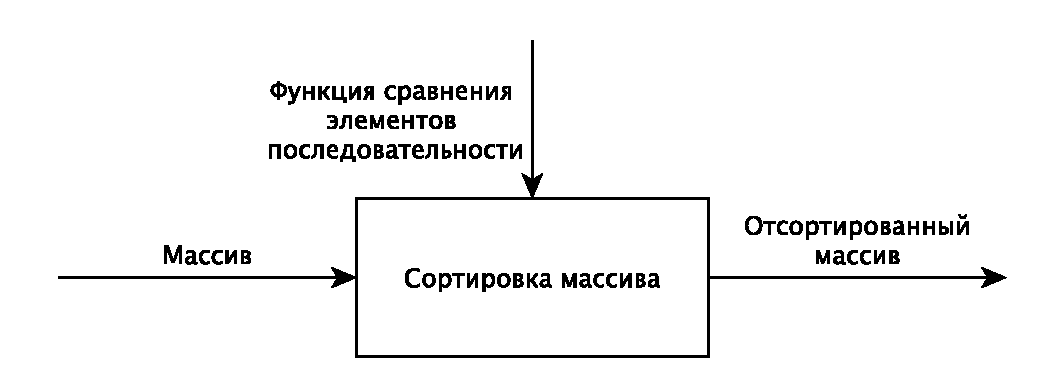
\includegraphics[scale = 0.8]{idef0} \\ Рис.  1 - Функциональная модель алгоритма сортировки. 
	\end{center}
	
        \subsection{Схемы алгоритмов}
        \hfill
        
        Приведем схемы 3 исследуемых алгоритмов (см. рисунки 2-4). 
        
        \paragraph{Поразрядная сортировка}
        
        \begin{center}
        		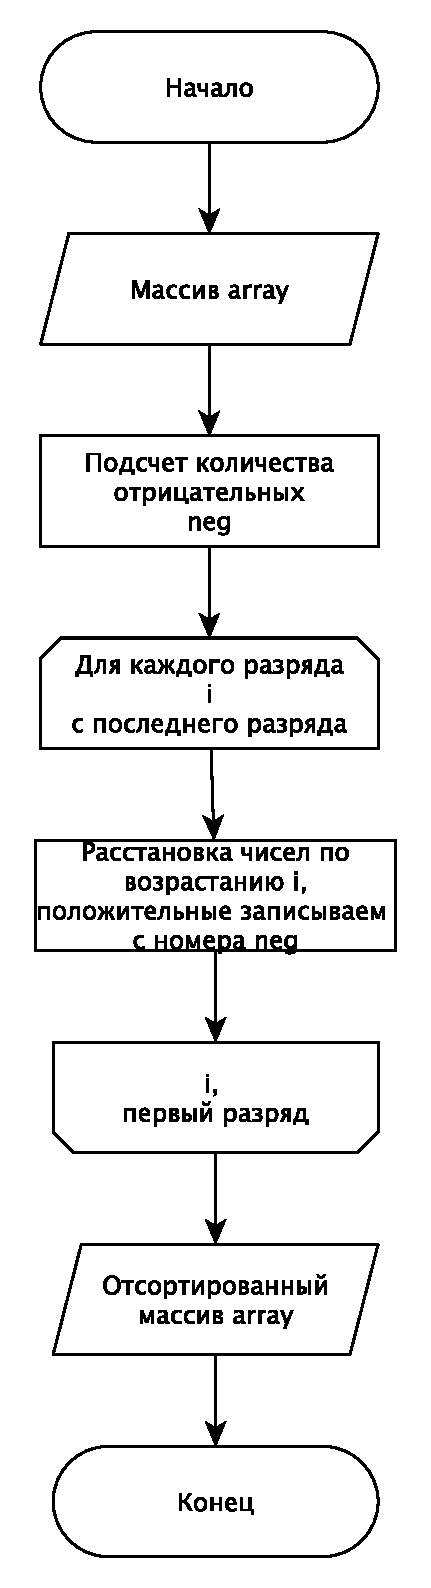
\includegraphics[scale = 0.8]{shema1} \\ Рис. 2 - Алгоритм поразрядной сортировки
	\end{center}
	
        \hfill
        \paragraph{Сортировка вставками}
        
        \begin{center}
        		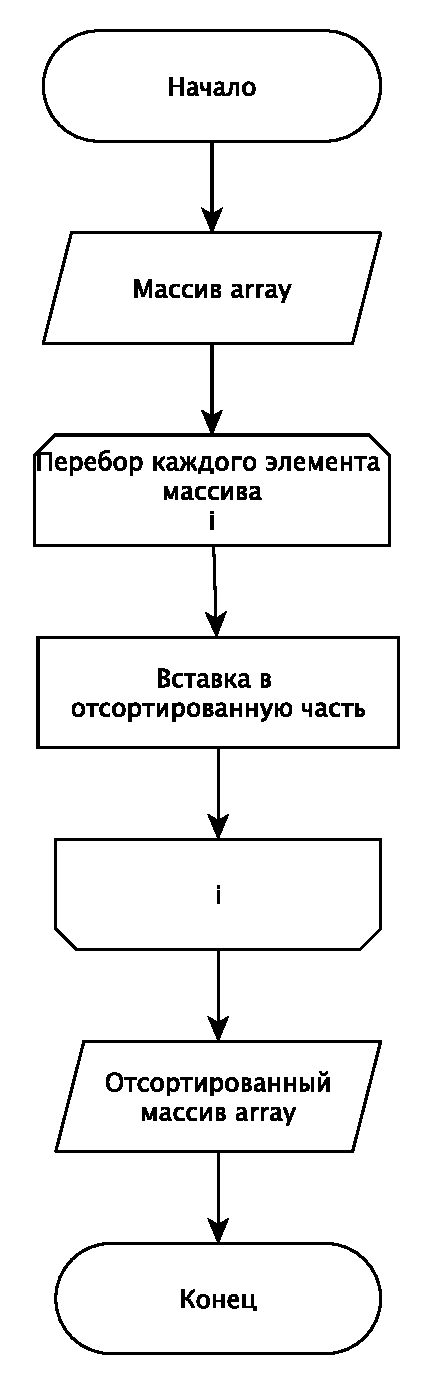
\includegraphics[scale = 0.8]{shema2} \\ Рис. 3 - Алгоритм сортировки вставками
	\end{center}
	
	\hfill
	\paragraph{Быстрая сортировка}
	
	\begin{center}
        		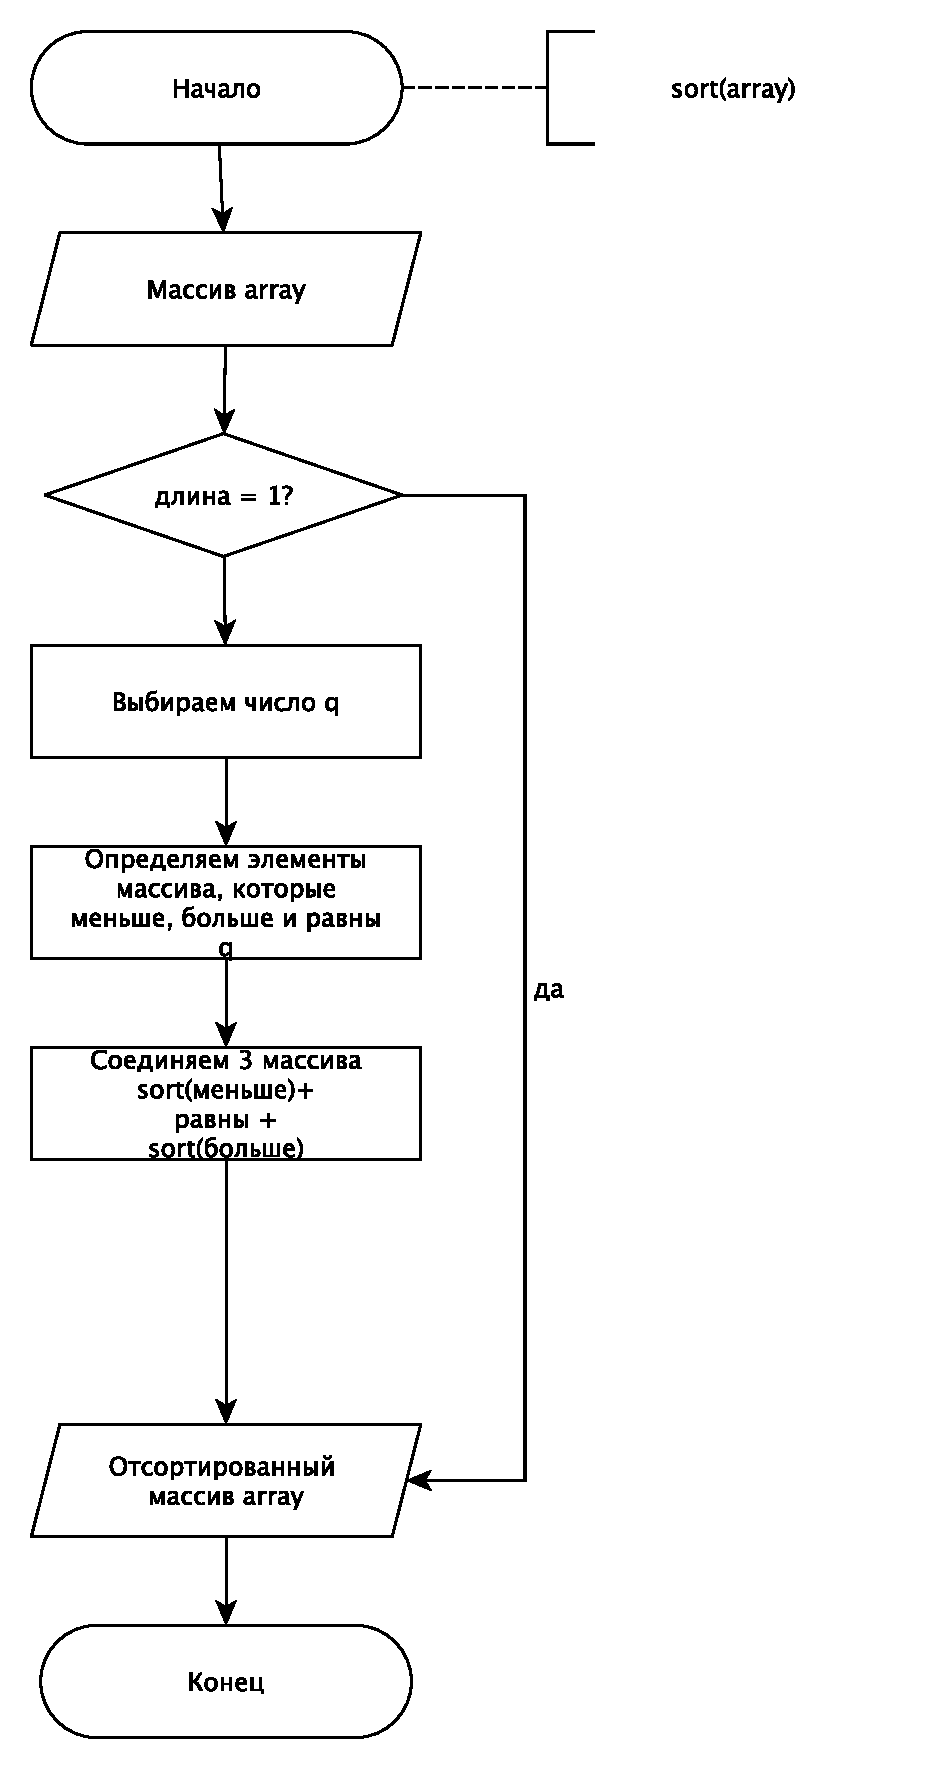
\includegraphics[scale = 0.8]{shema3} \\ Рис. 4 - Алгоритм быстрой сортировки
	\end{center}	
	
	\hfill
	
	\textbf{Произведем теоретическую оценку трудоемкости алгоритмов сортирвки}
	\begin{enumerate}
		\item Поразрядная сортировка 
		$$f=len + 2 + digit(2 +\underbrace{2 + len(2+1)}_{\text{расстановка}} + \underbrace{2 +digit(2+1)}_{\text{запись в массив}}=$$
		$$ = len+2 +digit(6+3len+2digit)=len+2+6digit+2digit^2+3digit\cdot len$$
		$$f = O(nk), n - \text{размер массива}, k- \text{порядок числа}$$
		$$\textbf{чем больше порядок числа тем больше трудоемкость}$$
		
		\item Сортировка вставками
		$$f=2+len(2+\underbrace{2+key(2+1)}_{\text{поиск позиции(сравнение)}}+\underbrace{1}_{\text{вставка}})=$$
		$$=2+len(5+3key)=2+5len+3len\cdot key$$
		$$f=O(n), n -\text{размер массива, }\textbf{Лучший случай - упорядоченный массив}$$
		$$f=O(n^2), n -\text{размер массива, }\textbf{Худший случай - обратноупорядоченный массив}$$
		$$f=O(n^2), n -\text{размер массива, }\textbf{Средний случай}$$
		
		\item Быстрая сортировка (из [7])
		$$f=O(n \cdot ln(n)),, n -\text{размер массива, }\textbf{Лучший случай- упорядоченный массив}$$
		$$f=O(n^2), n -\text{размер массива, }\textbf{Худший случай - обратноупорядоченный массив}$$
		$$f=O(n \cdot ln(n)), n -\text{размер массива, }\textbf{Средний случай}$$
	\end{enumerate}
	
       	\subsection{Выводы}
	\hfill
	
	Сортировка является одной из типовых проблем обработки данных и обычно понимается как задача размещения элементов неупорядоченного набора значений в порядке монотонного возрастания или убывания.
	
	Возможные способы решения этой задачи широко обсуждаются в литературе.
	
	Вычислительная трудоемкость процедуры упорядочивания является достаточно высокой. Так, для ряда известных простых методов (пузырьковая сортировка, сортировка включением и др.) количество необходимых операций определяется квадратичной зависимостью от числа упорядочиваемых данных. Для более эффективных алгоритмов трудоемкость ниже. 
	
	Однако для различных сортировок можно получить меньшую трудоемкость на частных вариантах задачи.
	
	\hfill
	
	В работе рассматриваются сортировки: поразрядная, вставками и быстрая. Наименьшей трудоемкостью обладает поразрядная сортировка, хотя в некоторых случаях быстрая сортировка будет у нее выигрывать. Рассмотрим это далее. 
	
    	\newpage

        \section{Технологическая часть}
        \hfill
        
        Стоит задача разработки и сравнительного анализа алгоритмов сортировки массивов.
        
        В реализациях в целях увеличения точности подсчета времени вывод массива был вынесен за пределы функций-алгоритмов. В целях наглядности были опущены части программ, не относящиеся к работе алгоритмов.
       
        \subsection{Требования к программному обеспечению}
        \hfill
        
        ПО должно предоставлять возможность замеров процессорного времени выполнения реализации каждого алгоритма. Требуется провести замеры для варьирующихся размеров массива до 10000 элементов. Один эксперимент ставится не менее 50 раз, результат одного эксперимента рассчитывается как среднее значение результатов проведенных испытаний с одинаковыми входными данными.
        \hfill
        
        \subsection{Средства реализации}
        \hfill
        
        В качестве языка программирования был выбран Python[8], так как я знакома с этих языком программирования. 
        \hfill
        
        Для замеров времени была выбран метод $process\_time()$, возвращает текущее время процессора как число с плавающей запятой, выраженное в секундах в Unix.
        \hfill
        
        Для генерации случайных чисел использовался метод $randint()$. 
        \hfill
        
        \subsection{Листинг кода}
        \hfill
        
        \textbf{Поразрядная сортировка:}
        
	\begin{lstlisting}
	n = pow(digit, n)
    	i = 1
    	while (i < n):
		sort = [[] for k in range(digit)]

		for x in array:
			sort[get_digit(x, i)].append(x)

		count = len(array)
		array = [0] * count
		u = 0
		w = 0
		for k in range(digit):
			for j in range(len(sort[k])):
				if (sort[k][j] < 0):
					array[w] = sort[k][j]
					w += 1
				else:
					array[u + neg] = sort[k][j]
					u += 1
		i *= 10
	\end{lstlisting}

	\textbf{Сортировка вставками: }
	
	\begin{lstlisting}
	for i in range(1, len(array)):
		j = i - 1
		key = array[i]
		while array[j] > key and j >= 0:
			array[j + 1] = array[j]
			j -= 1
		array[j + 1] = key
	\end{lstlisting}

	\textbf{Быстрая сортировка: }
	
	\begin{lstlisting}
def partition(nums, low, high):
    middle = nums[(low + high) // 2]
    i = low - 1
    j = high + 1
    while True:
        i += 1
        while nums[i] < middle:
            i += 1
        j -= 1
        while nums[j] > middle:
            j -= 1
        if i >= j:
            return j
        nums[i], nums[j] = nums[j], nums[i]

def quicking_sort(items, low, high):
    if low < high:
        split_index = partition(items, low, high)
        quicking_sort(items, low, split_index)
        quicking_sort(items, split_index + 1, high)

def quick_sort(nums):
    quicking_sort(nums, 0, len(nums) - 1)
        
	\end{lstlisting}
                
	\subsection{Тестирование}
	\hfill
	
	В таблице 1 представлена заготовка данных для тестирования наших алгоритмов. 
	\begin{center}
		\begin{tabular}{  | c | c | }
			\hline
			\textbf{Маcсив}& \textbf{Ожидаемый результат} \\ \hline
			$\begin{bmatrix} 
   			1&2&3 \\
			\end{bmatrix}$ & 
			$\begin{bmatrix} 
   			1&2&3 \\
			\end{bmatrix}$ \\
			\hline
			
			$\begin{bmatrix} 
   			3&2&1 \\
			\end{bmatrix}$ & 
			$\begin{bmatrix} 
   			1&2&3 \\
			\end{bmatrix}$ \\
			\hline
			
			$\begin{bmatrix} 
   			1&2&-3 \\
			\end{bmatrix}$ & 
			$\begin{bmatrix} 
   			-3&1&2 \\
			\end{bmatrix}$ \\
			\hline
			
			$\begin{bmatrix} 
   			1&0&-3 \\
			\end{bmatrix}$ & 
			$\begin{bmatrix} 
   			-3&0&1 \\
			\end{bmatrix}$ \\
			\hline
			
			$\begin{bmatrix} 
   			0 \\
			\end{bmatrix}$ & 
			$\begin{bmatrix} 
   			0 \\
			\end{bmatrix}$ \\
			\hline
		\end{tabular}
		
		\hfill
		
		Таблица 1.
		Подготовленные тестовые данные.  
	\end{center}

	
	\subsection{Выводы}
	\hfill
	
	Реализовано 3 алгоритма, подготовлены тесты для оценки качества их работы. 
        
        Получены практические навыки реализации алгоритмов сортировки: поразрядного, вставками и быстрого.
        
        \newpage

        \section{Экспериментальная часть}
                
    	\hfill
	
        Оценка качества работы алгоритмов. Экспериментальное сравнение работы различных алгоритмов (зависи- мость времени выполнения от размера массивов).
        
        \subsection{Примеры работы}
	\hfill
	
	На рисунке 5 представлены примеры работы программы на разных входных данных. 
	\begin{figure}[ht]\center
		\begin{tabular}{cc}
			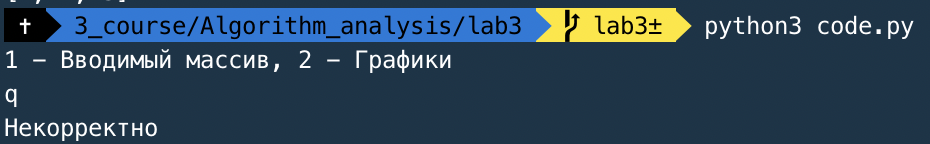
\includegraphics[width=80mm]{ex1} & 
\includegraphics[width=80mm]{ex2} \\
			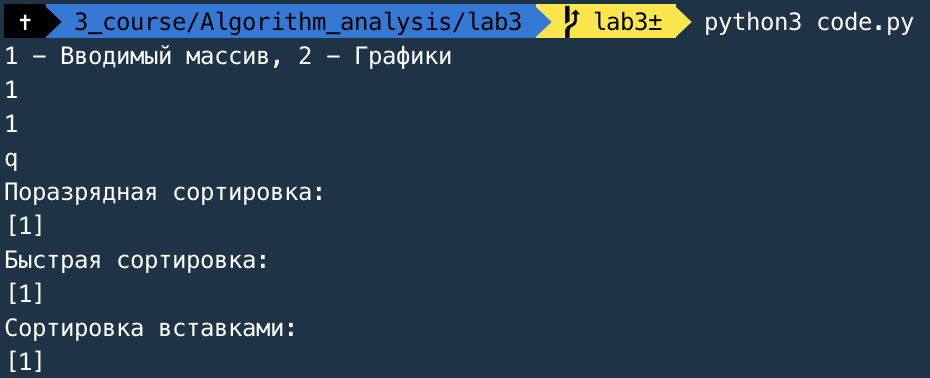
\includegraphics[width=80mm]{ex3} & 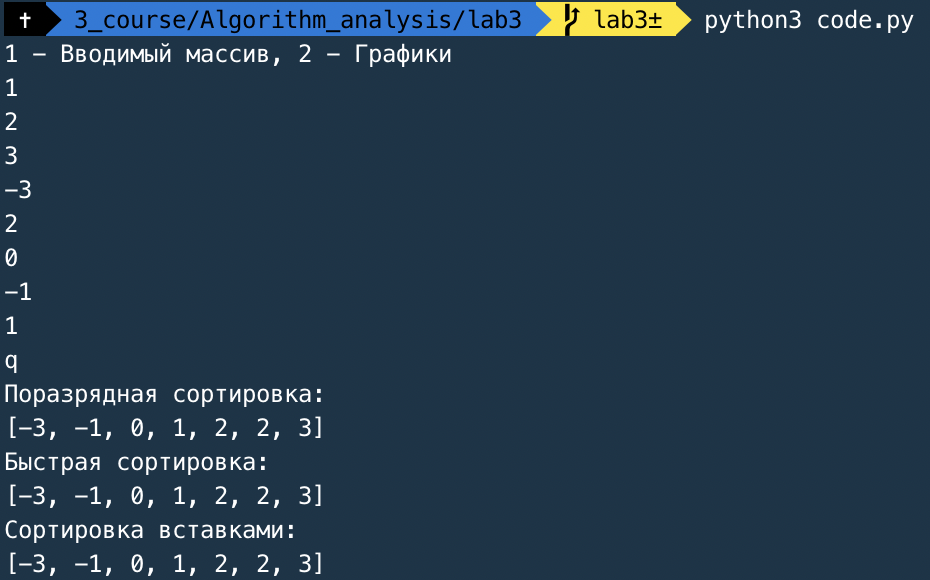
\includegraphics[width=80mm]{ex4}
		\end{tabular}
		\\ Рис. 5 - Примеры работы
	\end{figure}
	
	
	        
        \subsection{Результаты тестирования}
        
         Проверяем нашу программу на тестах из таблицы 1. Полученные результаты представлены в таблице 2. 
	\begin{center}
		\begin{tabular}{  | c | c | c | c |}
			\hline
			\textbf{Маcсив}& \textbf{Поразрядная сортировка} & \textbf{Быстрая сортировка} & \textbf{Сортировка вставками} \\ \hline
			$\begin{bmatrix} 
   			1&2&3 \\
			\end{bmatrix}$ & 
			$\begin{bmatrix} 
   			1&2&3 \\
			\end{bmatrix}$ 
			& 
			$\begin{bmatrix} 
   			1&2&3 \\
			\end{bmatrix}$
			& 
			$\begin{bmatrix} 
   			1&2&3 \\
			\end{bmatrix}$ \\
			\hline
			
			$\begin{bmatrix} 
   			3&2&1 \\
			\end{bmatrix}$ & 
			$\begin{bmatrix} 
   			1&2&3 \\
			\end{bmatrix}$ & 
			$\begin{bmatrix} 
   			1&2&3 \\
			\end{bmatrix}$ & 
			$\begin{bmatrix} 
   			1&2&3 \\
			\end{bmatrix}$ \\
			\hline
			
			$\begin{bmatrix} 
   			1&2&-3 \\
			\end{bmatrix}$ & 
			$\begin{bmatrix} 
   			-3&1&2 \\
			\end{bmatrix}$ & 
			$\begin{bmatrix} 
   			-3&1&2 \\
			\end{bmatrix}$ & 
			$\begin{bmatrix} 
   			-3&1&2 \\
			\end{bmatrix}$ \\
			\hline
			
			$\begin{bmatrix} 
   			1&0&-3 \\
			\end{bmatrix}$ & 
			$\begin{bmatrix} 
   			-3&0&1 \\
			\end{bmatrix}$ & 
			$\begin{bmatrix} 
   			-3&0&1 \\
			\end{bmatrix}$ & 
			$\begin{bmatrix} 
   			-3&0&1 \\
			\end{bmatrix}$ \\
			\hline
			
			$\begin{bmatrix} 
   			0 \\
			\end{bmatrix}$ & 
			$\begin{bmatrix} 
   			0 \\
			\end{bmatrix}$ & 
			$\begin{bmatrix} 
   			0 \\
			\end{bmatrix}$ & 
			$\begin{bmatrix} 
   			0 \\
			\end{bmatrix}$ \\
			\hline
		\end{tabular}
		
		\hfill
		
		Таблица 2.
		Тестирование программы.   
	\end{center}
        
	\hfill
		
	
	\textbf{Тесты пройдены}

	\subsection{Замеры времени}
	\hfill
	
	На графиках 6-11 представлено сравнение алгоритмов сортировки массивов. 
	\begin{center}
        		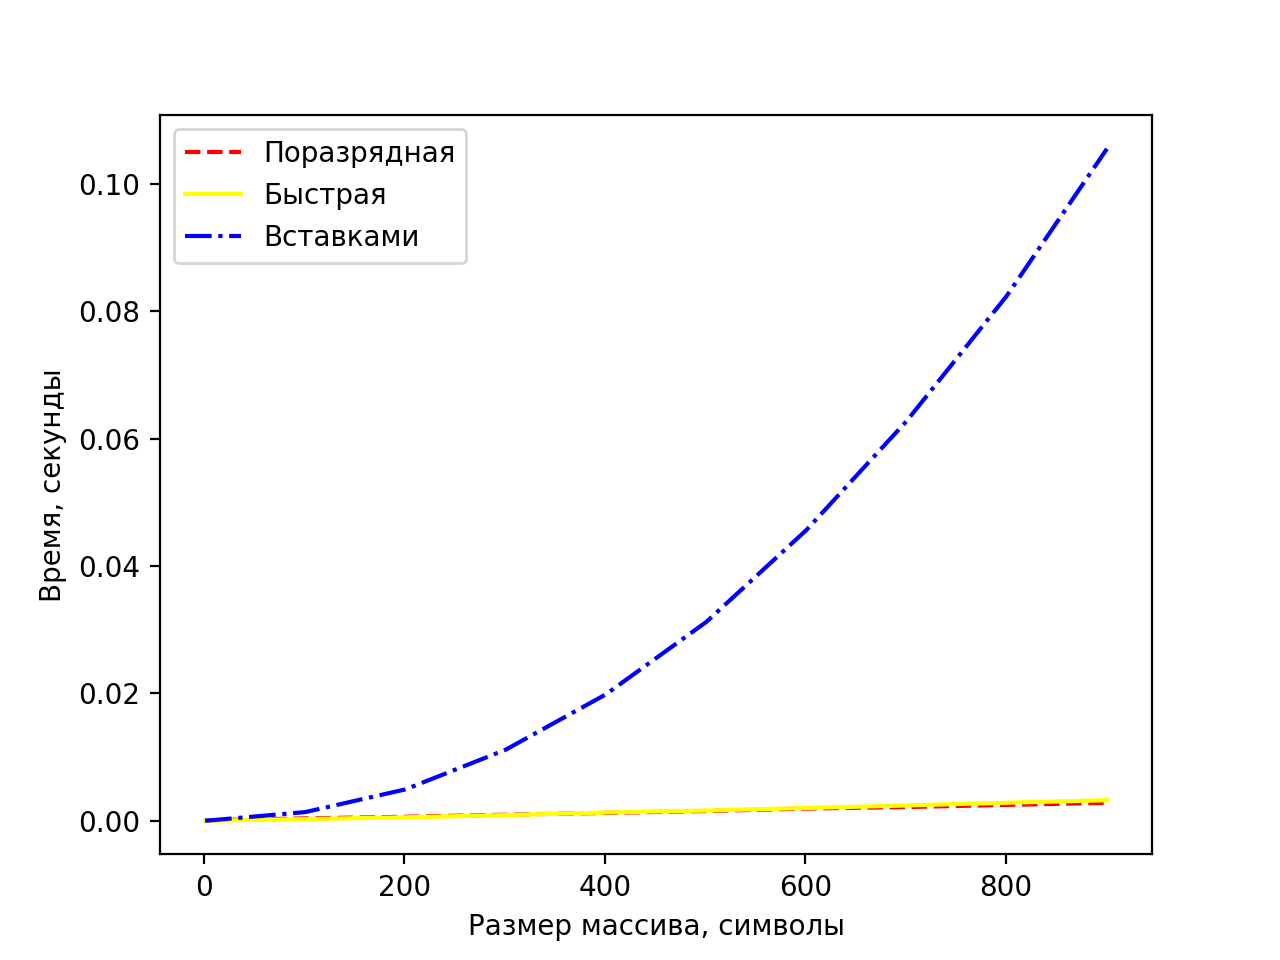
\includegraphics[scale = 1]{graph1} \\ Рис. 6 - Сравнение реализации алгоритмов сортировок на произвольных данных
	\end{center}
	
	Как видно из графика 6, сортировка вставками должна рассматриваться отдельно от быстрой и поразрядной, так как ее трудоемкость очень высока. 
	
	\begin{center}
        		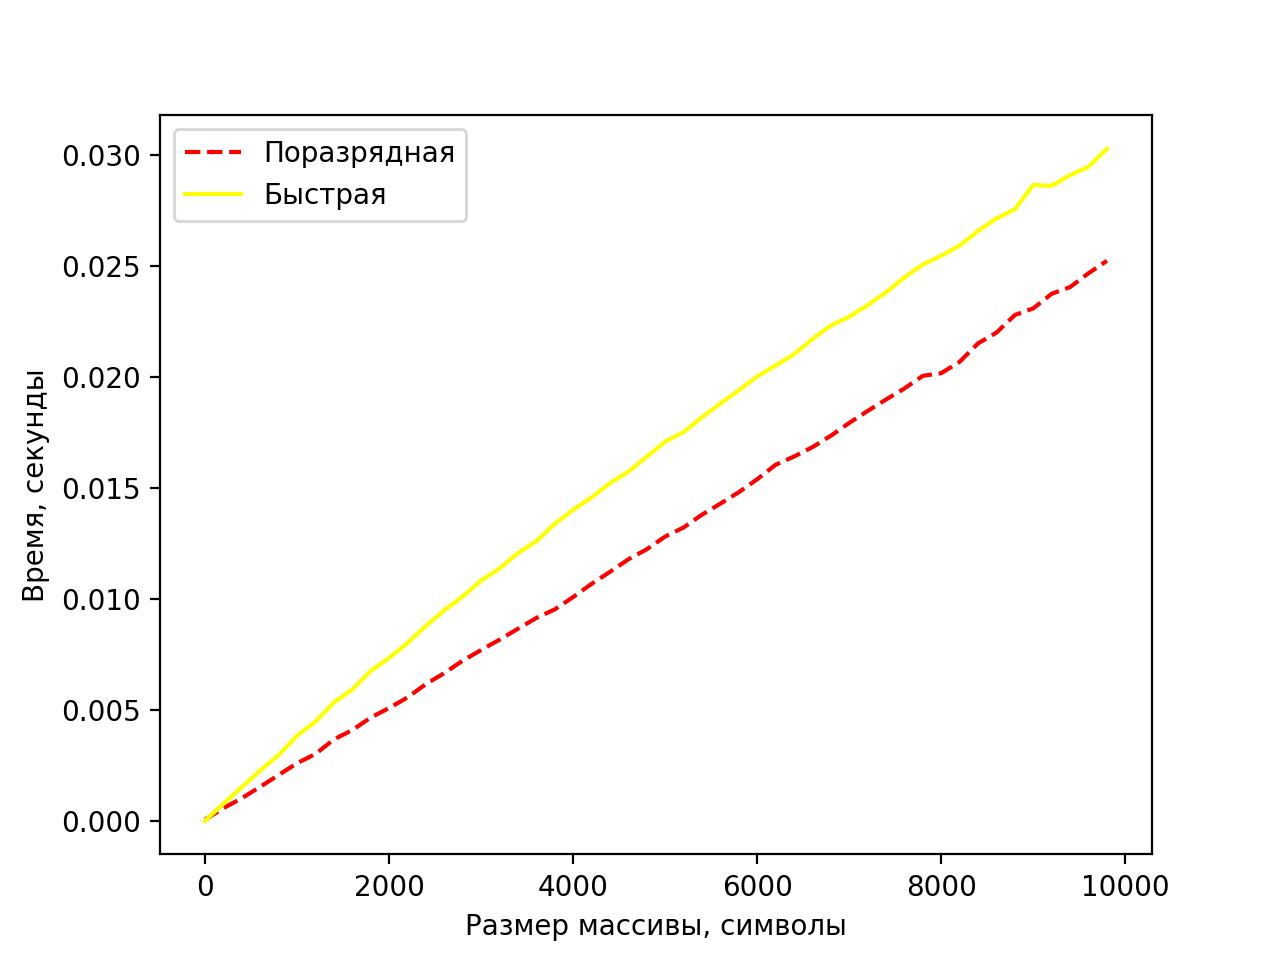
\includegraphics[scale = 1]{graph2} \\ Рис. 7 - Сравнение реализации алгоритмов сортировок быстрой и поразрядной на произвольных данных (при средней разрядности числа до 4 значащих цифр)
	\end{center}
	
	\begin{center}
        		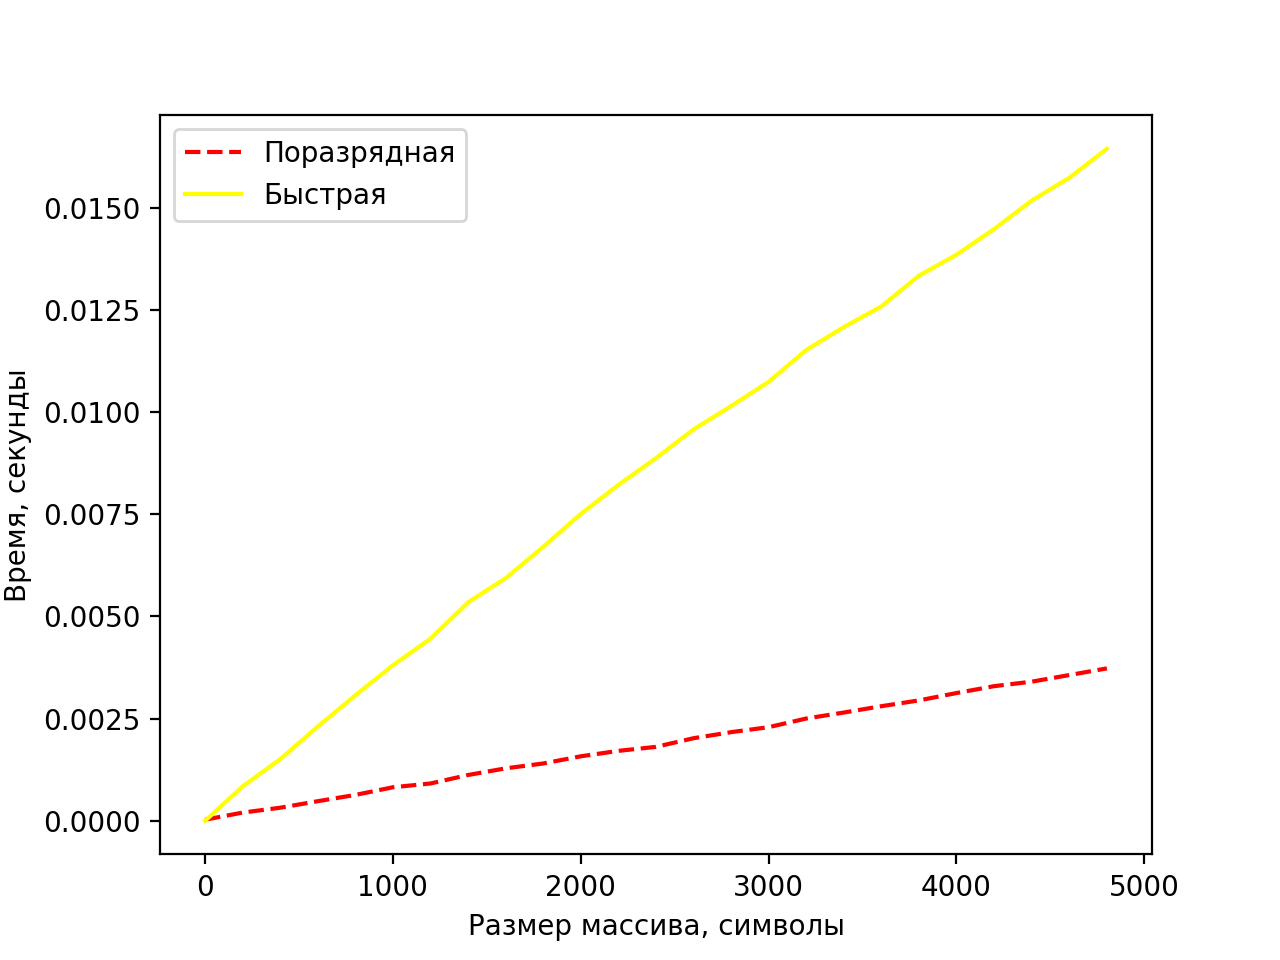
\includegraphics[scale = 1]{graph3} \\ Рис. 8 - Сравнение реализации алгоритмов сортировок быстрой и поразрядной на произвольных данных (при маленькой разрядности числа 1 значащая цифра)
	\end{center}
	
	\begin{center}
        		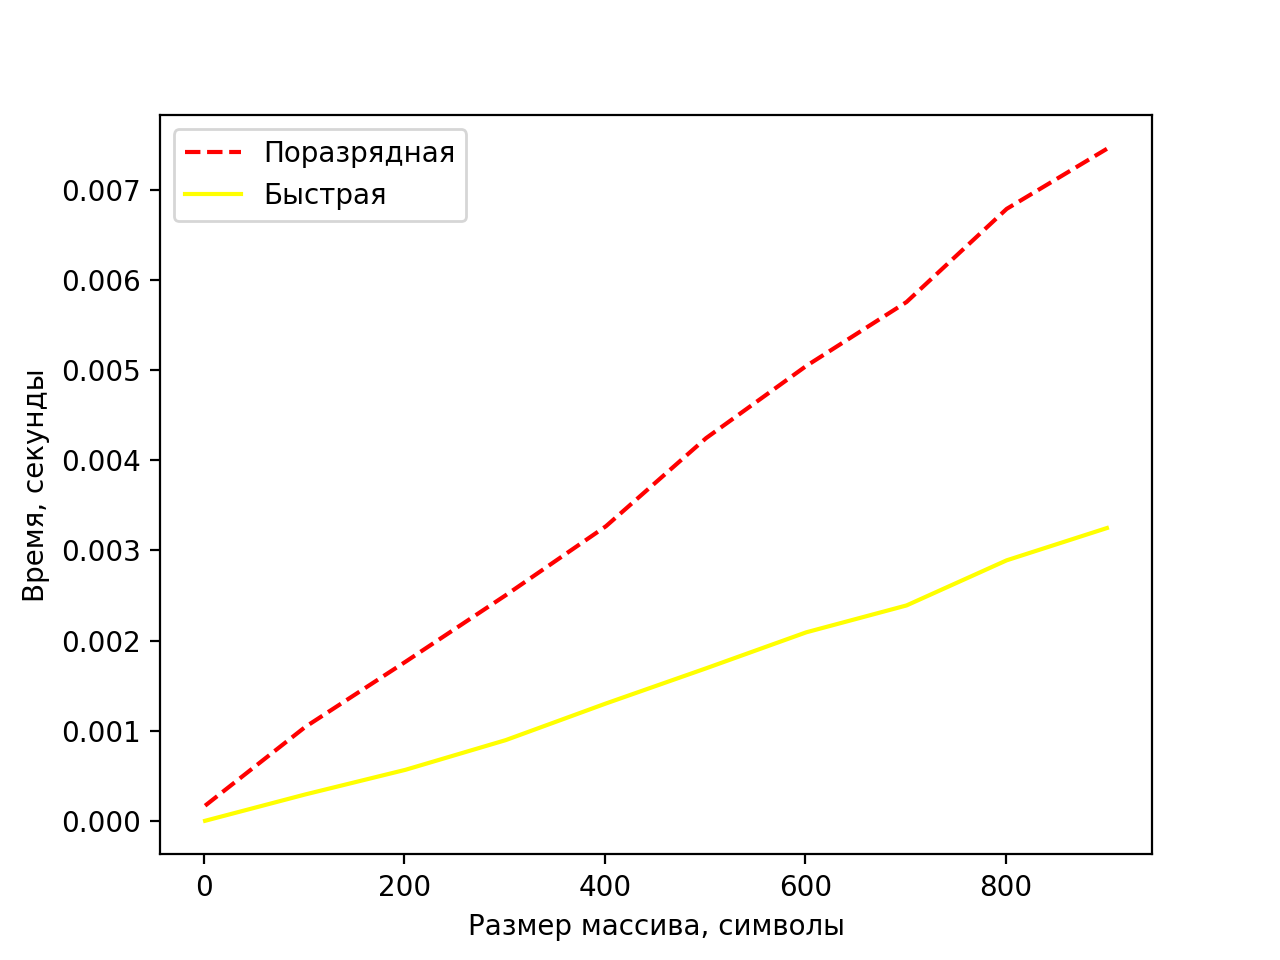
\includegraphics[scale = 1]{graph4} \\ Рис. 9 - Сравнение реализации алгоритмов сортировок быстрой и поразрядной на произвольных данных (при большой разрядности числа до 10 значащих цифр)
	\end{center}
	
	\begin{center}
        		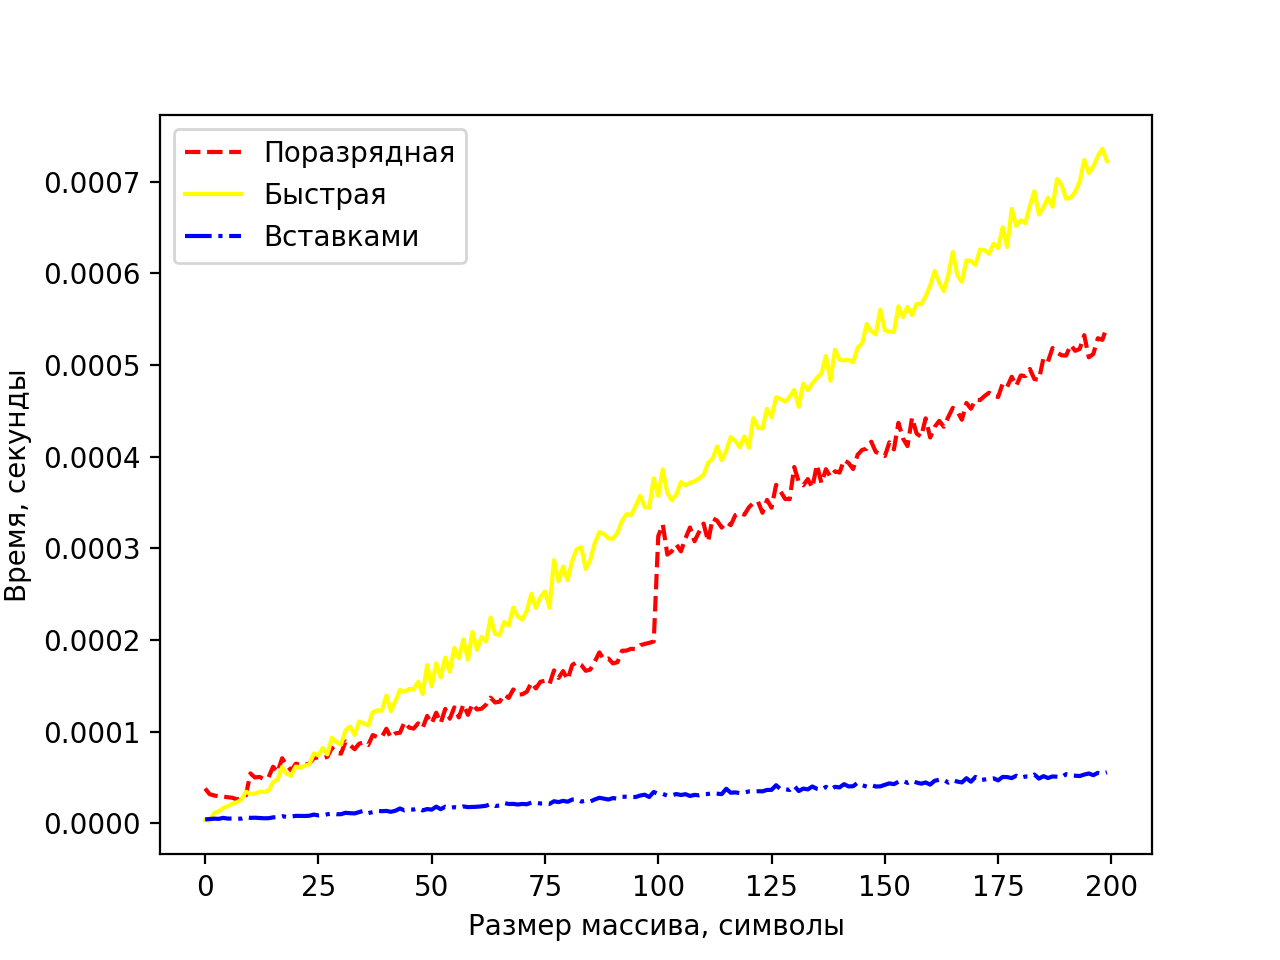
\includegraphics[scale = 1]{graph5} \\ Рис. 10 - Сравнение реализации алгоритмов сортировок на упорядоченных данных
	\end{center}
	
	\begin{center}
        		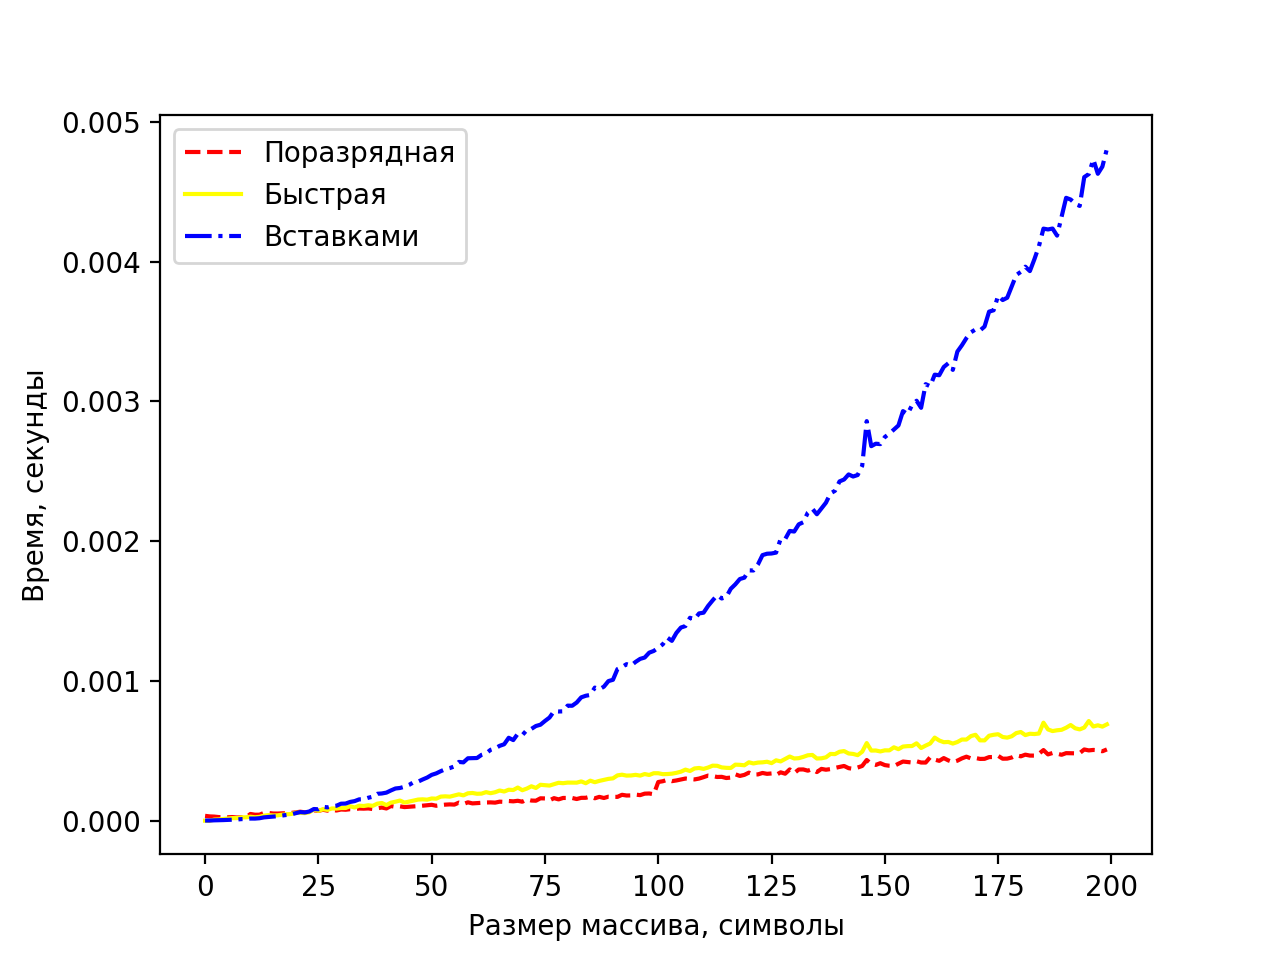
\includegraphics[scale = 1]{graph6} \\ Рис. 11 - Сравнение реализации алгоритмов сортировок на обратно упорядоченных данных
	\end{center}
	
	\begin{center}
        		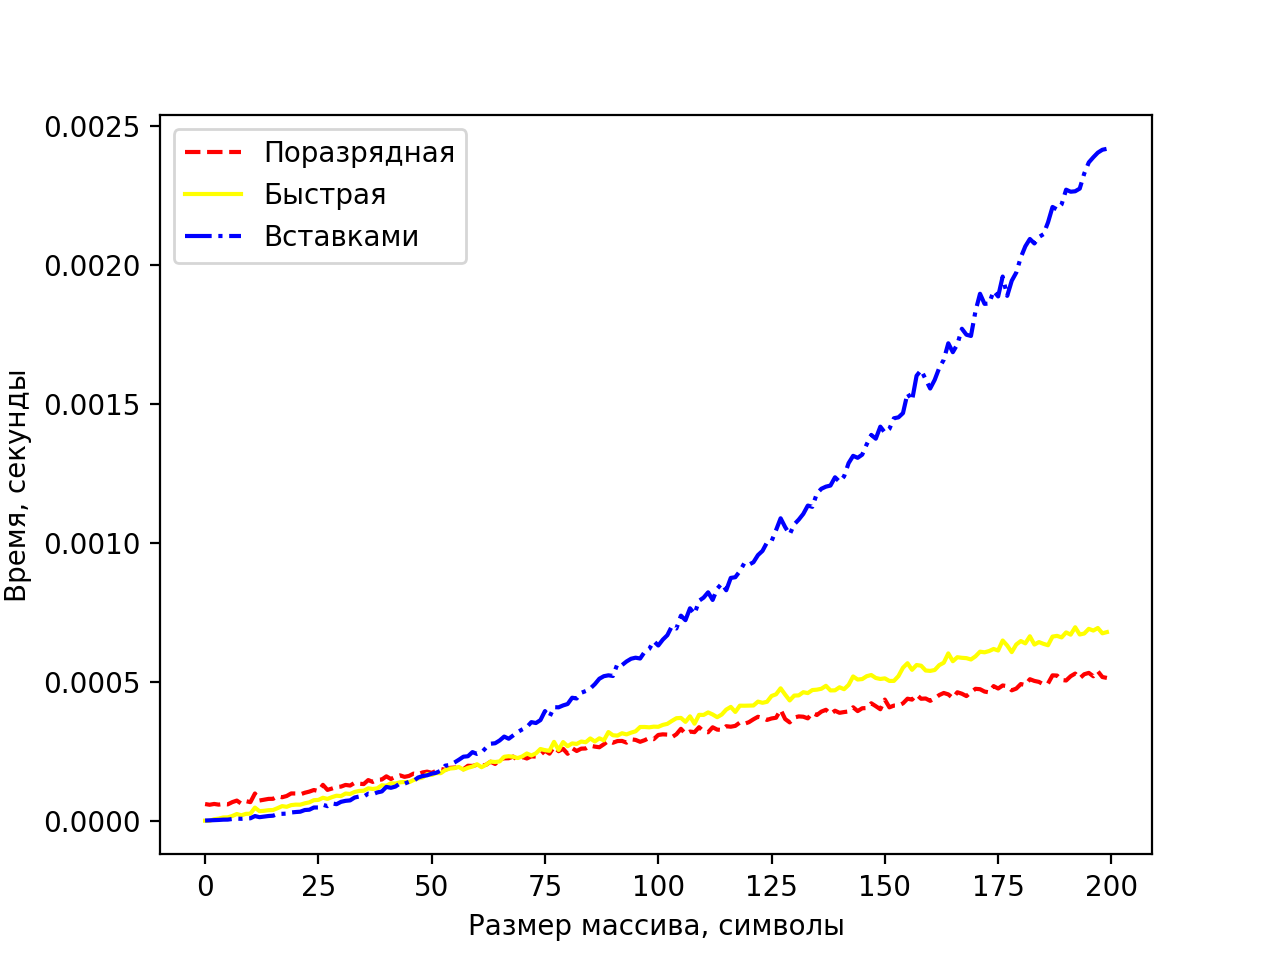
\includegraphics[scale = 1]{graph7} \\ Рис. 12 - Сравнение реализации алгоритмов сортировок на произвольных данных при небольших размерах массивов
	\end{center}
	
		
	\subsection{Выводы}
	\hfill
	
	Таким образом, по графикам подтвердилось предположение, о том, что самыми эффективным по скорости работы являются поразрядный алгоритм и быстрая сортировка. При размерностях выше $ln(n)$ (из оценки трудоемкости, где n - длина массива) быстрая сортировка оказывается эффективнее. 
	
	Также, оказалось, что при размерах массива меньше 50 эффективнее использовать сортировку вставками. 
	
   	\newpage

        \anonsection{Заключение}
        
        \hfill
        
         В данной работе был проведен обзор 3 популярных алгоритмов сортировки. 
	\begin{enumerate}
		\item Изучены алгоритмы сортировки массивов данных: быстрая сортировка, сортировка вставками и поразрядная сортировка. 
		\item Произведена оценка трудоемкости алгоритмов для лучших и худших и случаев и условий их наступления. 
		\item Получены практические навыки реализации алгоритмов сортировки на одном из языков программирования. 
		\item Проведен сравнительный анализ алгоритмов по затрачиваемым ресурсам (зависимость времени от длины массива)
		\item Экспериментально подтверждены различия в трудоемкости алгоритмов с указанием лучших и худших случаев. 
	\end{enumerate}
	
	При сравнении данных алгоритмов пришли к следующим выводам:
	\begin{enumerate}
 		\item Самым эффективным на средних наборах данных (числа разрядностью до 4 знаков) является алгоритм поразрядной сортировки. Однако при размерах массива меньших 50 рекомендуется использовать алгоритм сортировки вставками (или другие алгоритмы квадратичной сложности). 
		
 		\item Быстрая сортировка является эффективной при больших размерах массивов (больших 50) и при разрядности чисел больших 4. 
		
	\end{enumerate}
	
 	\newpage

        \begin{thebibliography}{}
        		\bibitem{} Сортировка и фильтрация таблицы [Электронный ресурс]. - Режим доступа: https://support.office.com/ru-ru/article/Сортировка-и-фильтрация-таблицы-в-excel-с-помощью-средства-чтения-с-экрана-d6ae119c-5fab-4b7f-8869-6ef02ece71f5 (дата обращения: 19.10.2019)
		\bibitem{} Кнут Д. Э., Козаченко Ю. В., Красиков И. В. Искусство программирования: Сортировка и поиск. Классический труд, Т. 3. М. : Вильямс, 2000. –– 824 c.
		\bibitem{}  Sorting Benchmarks [Электронный ресурс]. - Режим доступа: http://sortbenchmark.org/ (дата обращения: 19.10.2019)
		\bibitem{}  Алгоритмы сортировки [Электронный ресурс]. - Режим доступа: http://kit.znu.edu.ua/Meth/SORTALG.pdf (дата обращения: 19.10.2019)
		\bibitem{} Алгоритм сортировки [Электронный ресурс]. - Режим доступа: https://www.wikiwand.com/ru/Алгоритмсортировки (дата обращения: 19.10.2019)
		\bibitem{}  Алгоритмы сортировки в народных танцах [Электронный ресурс]. - Режим доступа: https://forany.xyz/a-370 (дата обращения: 19.10.2019)
		\bibitem{}  Сортировка данных [Электронный ресурс]. - Режим доступа: http://www.hpcc.unn.ru/mskurs/RUS/DOC/ppr10.pdf (дата обращения: 19.10.2019)
	\end{thebibliography} 

\end{document}
